\documentclass[11pt]{article}

\usepackage[margin=1in]{geometry}
\usepackage{amsmath, amssymb, amsthm}
\usepackage{graphicx}
\usepackage{hyperref}

\title{A Practical On-Chain Gaussian Sampler from VM-Native Bit-Count Transforms}
\author{Simon Tian}
\date{}

\newtheorem{theorem}{Theorem}
\newtheorem{remark}{Remark}

\begin{document}

\maketitle

\begin{abstract}
This paper studies a practical Gaussian sampler for on-chain use built from the
count of $1$'s in an $n$-bit VM-native output. The construction is intentionally
simple: obtain an $n$-bit hash or randomness value, count the $1$'s in the
output, standardize that count, and represent the result as an integer-scaled
Gaussian approximation in a smart-contract VM. The probabilistic model treats
the output bits as independent Bernoulli random variables with possibly
different success probabilities. Under this model, the count of $1$'s is
Poisson-binomial, and Lyapunov's central limit theorem implies that the
standardized count is asymptotically Gaussian. Because practical VMs expose
concrete finite widths, the paper presents a detailed numerical study for
\texttt{keccak256} at $n=256$ and a cross-VM numerical expansion covering
Keccak-256, SHA-256, and Sui-native-randomness reference models at $n=256$ and
$n=512$. The empirical results do not prove independence, fairness, or
cryptographic suitability, but they do support a practical working model in
which the bit probabilities are close to $0.5$, the centering and scaling are
close to $(n/2, \sqrt{n}/2)$, the popcount distribution is close to a Gaussian
benchmark, and repeated-primitive sequences do not display obvious short-lag
structure in the tested regimes.
\end{abstract}

\section{Introduction}

Generating Gaussian-like random variables directly on-chain is awkward because
the usual floating-point transforms are expensive and do not map naturally to
smart-contract VMs. The construction studied here uses a simpler route. Given
an $n$-bit VM-native output, let $S_n$ denote the number of $1$'s in its bits.
If those bits behave like approximately independent Bernoulli variables with
success probabilities near $0.5$, then $S_n$ should be close to a Gaussian law
after centering and scaling.

This note combines the probabilistic argument and the numerical study into a
single paper so that the claims are presented as one continuous argument rather
than as two disconnected notes. The point is not to prove a theorem about the
internal structure of \texttt{keccak256}. The point is narrower: to justify a
practical on-chain Gaussian approximation under a clearly stated probabilistic
model, and to test whether the observed finite-sample behavior of
\texttt{keccak256} outputs is compatible with that model.

The main contributions are:
\begin{enumerate}
\item a simple integer-scaled Gaussian sampler construction based on the
popcount of VM-native outputs;
\item a Lyapunov-CLT justification for heterogeneous Bernoulli bit marginals;
\item a numerical study of bit-wise fairness, pairwise dependence, input-output
structure, popcount normality, and repeated-hash sequence behavior.
\item a cross-VM applicability analysis showing that the method has direct
relevance for EVM and Solana as missing-Gaussian-primitive targets, and for
Sui as a Gaussianization layer over native on-chain randomness.
\end{enumerate}

\section{Cross-VM Applicability}

The construction in this paper should be read as a \emph{Gaussianization layer}
for VM-exposed cryptographic primitives. The entropy source itself is outside
the scope of the paper. In practice, that source could come from beacon
randomness, native randomness services, or external systems such as VRFs. Once a
VM makes a suitable unpredictable seed available, the contribution of this
paper is to transform that seed into a lightweight on-chain Gaussian-like draw.

Under that framing, EVM, Solana, and Sui play different roles.

\textbf{EVM.} EVM chains are the primary target. Solidity exposes the relevant
hash functions directly, and modern EVM chains also expose
\texttt{block.prevrandao} as a randomness input. What the VM does \emph{not}
expose is a native Gaussian random primitive. This makes the present method a
direct fit for Ethereum and EVM-compatible chains.

\textbf{Solana.} Solana is the strongest non-EVM target. The SVM exposes native
hashing syscalls including SHA-256, Keccak-256, and Blake3. At the same time,
Solana's programming model remains deterministic and does not provide native
on-chain randomness in the same sense as a built-in random object; developers
are pushed toward VRF-style integrations for entropy. This makes the proposed
transform attractive as a lightweight Gaussian sampler once an external entropy
source has been imported.

\textbf{Sui.} Sui differs from the previous two systems because it already
provides native on-chain randomness through \texttt{Random} and
\texttt{RandomGenerator}. However, the documented API is aimed at generating
uniform values and values in explicit ranges. It does not document a native
Gaussian or normal-distribution primitive. Therefore Sui is still a meaningful
target for this method, not because it lacks randomness altogether, but because
it still lacks an equally lightweight native Gaussian sampler layered on top of
its native randomness service.

\begin{table}[htbp]
\centering
\small
\begin{tabular}{llll}
\hline
VM & Native primitive & Randomness status & Role in this paper \\
\hline
EVM & Keccak-256, SHA-256 & no native Gaussian primitive & primary target \\
Solana & SHA-256, Keccak-256, Blake3 & external entropy needed & primary target \\
Sui & RandomGenerator & native randomness exists & Gaussian layer target \\
\hline
\end{tabular}
\caption{Target selection for the cross-VM version of the method.}
\label{tab:vm-scope}
\end{table}

\section{Generator Construction}

Let $H_n$ be an $n$-bit value produced by a VM-native primitive. Write its
output bits as
\[
X_{n,1}, X_{n,2}, \dots, X_{n,n},
\]
where $X_{n,i} = 1$ if the $i$-th bit is $1$ and $X_{n,i} = 0$ otherwise.
Define
\[
S_n = \sum_{i=1}^{n} X_{n,i},
\]
the count of $1$'s in the digest.

The natural Gaussian approximation used throughout this paper is
\[
Y_n = \frac{S_n - n/2}{\sqrt{n}/2}.
\]

Because smart-contract VMs do not natively support floating-point arithmetic,
the contract-level output can instead be represented at integer scale $c$ by
\[
Z_{n,c} = \operatorname{round}(cY_n).
\]

Two concrete examples are especially relevant here.
\begin{enumerate}
\item For a 256-bit primitive, such as Keccak-256 or SHA-256,
\[
Y_{256} = \frac{S_{256} - 128}{8},
\]
and with $c = 1000$ this becomes the exact integer formula
\[
Z_{256,1000} = 125S_{256} - 16000.
\]
\item For a 512-bit primitive or a 512-bit randomness sample,
\[
Y_{512} = \frac{S_{512} - 256}{8\sqrt{2}},
\]
and with $c = 1000$ the on-chain integer representation is
\[
Z_{512,1000} = \operatorname{round}\left(\frac{1000(S_{512}-256)}{8\sqrt{2}}\right).
\]
\end{enumerate}

When multiple values are needed, the generator can be iterated by repeated
hashing. Starting from a seed,
\[
H_{n,1} = \mathcal{P}(\text{seed}),
\qquad
H_{n,t+1} = \mathcal{P}(H_{n,t}),
\]
where $\mathcal{P}$ is the selected VM-native primitive, and each output is
derived from the corresponding popcount
\[
S_{n,t} = \sum_{i=1}^{n} X_{n,t,i}.
\]

\section{Probabilistic Model}

The strongest defensible probabilistic model for this construction is not the
exact iid Bernoulli$(0.5)$ model. Instead, let
\[
X_{n,1}, \dots, X_{n,n}
\]
be independent Bernoulli random variables with bit-specific success
probabilities
\[
\mathbb{P}(X_{n,i}=1)=p_{n,i}.
\]
The values $p_{n,i}$ are allowed to vary with $i$ and need only be close to
$0.5$ in practice.

Under this model,
\[
S_n = \sum_{i=1}^n X_{n,i}
\]
has a Poisson-binomial distribution, with mean and variance
\[
\mu_n = \sum_{i=1}^n p_{n,i},
\qquad
\sigma_n^2 = \sum_{i=1}^n p_{n,i}(1-p_{n,i}).
\]
The natural standardized count is therefore
\[
Z_n = \frac{S_n - \mu_n}{\sigma_n}.
\]

The numerical study in this paper is intended to support, not prove, the use of
this model. In particular, it looks for empirical evidence against strong
bit-level bias, simple cross-bit dependence, simple input-output dependence, and
short-lag dependence in repeated-hash output sequences.

\section{Lyapunov-CLT Justification}

\begin{theorem}
Suppose that for each $n$, the family
\[
X_{n,1}, \dots, X_{n,n}
\]
consists of independent Bernoulli random variables with success probabilities
$p_{n,1}, \dots, p_{n,n}$. Assume there exists a constant
$\varepsilon \in (0, 1/2)$ such that
\[
\varepsilon \le p_{n,i} \le 1-\varepsilon
\]
for all relevant $n$ and $i$. Then Lyapunov's condition holds for $\delta=1$,
and
\[
\frac{S_n - \mu_n}{\sigma_n}
\xrightarrow{d}
\mathcal{N}(0,1)
\qquad \text{as } n \to \infty.
\]
\end{theorem}

\begin{proof}
For a Bernoulli random variable,
\[
\mathbb{E}\left[\left|X_{n,i} - p_{n,i}\right|^3\right]
= p_{n,i}(1-p_{n,i})^3 + (1-p_{n,i})p_{n,i}^3.
\]
The right-hand side is maximized at $p_{n,i}=1/2$, so
\[
\mathbb{E}\left[\left|X_{n,i} - p_{n,i}\right|^3\right] \le \frac{1}{8}.
\]
Hence
\[
\sum_{i=1}^n \mathbb{E}\left[\left|X_{n,i} - p_{n,i}\right|^3\right] = O(n).
\]

On the other hand,
\[
p_{n,i}(1-p_{n,i}) \ge \varepsilon(1-\varepsilon),
\]
so
\[
\sigma_n^2 = \sum_{i=1}^n p_{n,i}(1-p_{n,i}) \ge n\varepsilon(1-\varepsilon).
\]
Therefore
\[
\sigma_n^3 \ge \left(n\varepsilon(1-\varepsilon)\right)^{3/2},
\]
and the Lyapunov ratio is
\[
\frac{1}{\sigma_n^3}
\sum_{i=1}^n \mathbb{E}\left[\left|X_{n,i} - p_{n,i}\right|^3\right]
= O(n^{-1/2}) \to 0.
\]
Lyapunov's central limit theorem then gives the claim.
\end{proof}

For a practical VM primitive with output width $n$, the theorem is asymptotic,
so the finite-width use case still needs a finite-sample argument. The
practical bridge is empirical: if the numerical study indicates that the $p_i$
are close to $0.5$ and that obvious dependence is not detected, then
\[
\mu_n = \sum_{i=1}^{n} p_i \approx \frac{n}{2},
\qquad
\sigma_n^2 = \sum_{i=1}^{n} p_i(1-p_i) \approx \frac{n}{4},
\]
and the practical normalization
\[
\frac{S_n-n/2}{\sqrt{n}/2}
\]
should be close to the theoretically natural normalization
\[
\frac{S_n-\mu_n}{\sigma_n}.
\]

Writing
\[
p_i = \frac{1}{2} + e_i,
\]
gives
\[
\mu_n = \frac{n}{2} + \sum_{i=1}^{n} e_i,
\qquad
\sigma_n^2 = \frac{n}{4} - \sum_{i=1}^{n} e_i^2.
\]
This makes the main approximation transparent: the variance error is
second-order in the bit biases.

In the two concrete widths studied later in the paper, this gives
\[
(\mu_{256}, \sigma_{256}) \approx (128, 8)
\qquad \text{and} \qquad
(\mu_{512}, \sigma_{512}) \approx (256, 8\sqrt{2}).
\]

\section{Numerical Study Design}

The numerical study uses six one-shot input families:
\begin{enumerate}
\item sequential \texttt{uint256} values;
\item sequential \texttt{uint256} values shifted by $2^{128}$;
\item sequential strings of the form \texttt{Transaction Number: i};
\item shifted strings of the form \texttt{Transaction Number: }$2^{128}+i$;
\item random ASCII strings with length between $2$ and $7$;
\item random ASCII strings with length between $2$ and $32$.
\end{enumerate}

Each family contains $10{,}000$ hashes. For these families the study records:
\begin{enumerate}
\item bit-wise empirical means;
\item pairwise similarity and correlation diagnostics;
\item input-bit correlations for the sequential families;
\item bit-level autocorrelation summaries up to lag $30$;
\item popcount normalization and Gaussian-fit diagnostics.
\end{enumerate}

To study the recursive generator directly, the paper also evaluates four
repeated-hash chains of length $10{,}000$, started from representative integer
and string seeds. For these chains it records popcount autocorrelation, lag-1
scatter, runs-test $z$-scores, and tail error relative to the Gaussian
benchmark.

\section{Expanded Multi-VM Study}

The current numerical results in this paper are specific to
\texttt{keccak256}. For a cross-VM version of the paper, the study should be
expanded at the level of \emph{VM-exposed primitives} rather than at the level
of chain labels alone.

The cleanest study matrix is:
\begin{enumerate}
\item \textbf{Keccak-256:} shared VM-native primitive for EVM and Solana;
\item \textbf{SHA-256:} shared VM-native primitive for EVM and Solana;
\item \textbf{Sui native-randomness integration:} idealized 256-bit and
512-bit reference outputs representing direct Gaussianization targets for
\texttt{RandomGenerator}.
\end{enumerate}

Keeping a generic $n$-bit representation is important because it preserves the
same normalization template
\[
\frac{S_n-n/2}{\sqrt{n}/2}.
\]
This keeps the probabilistic framing unchanged even when concrete VMs expose
different widths.

For each primitive, the study should rerun the same diagnostics used in the
present \texttt{keccak256} analysis:
\begin{enumerate}
\item bit-wise bias and implied $(\hat\mu, \hat\sigma)$;
\item pairwise binary-sequence similarity and correlation diagnostics;
\item input-output correlation for structured input families;
\item bit-level autocorrelation;
\item popcount CDF, QQ, and tail diagnostics;
\item repeated-primitive sequence diagnostics;
\item execution-cost measurements in the native VM.
\end{enumerate}

The pairwise binary-sequence diagnostics are particularly important in the
cross-VM version. The original study already emphasized Rogers-Tanimoto,
Sokal-Michener, and phi-correlation as structure-sensitive checks on binary
outputs before collapsing them into a scalar popcount. Those same diagnostics
should be preserved for every VM primitive in the expanded study.

Figure~\ref{fig:cross-vm-overview} summarizes the worst observed centering
error, scaling error, Kolmogorov-Smirnov distance, and two-sided tail error at
$z=2$ across the expanded cross-VM targets. Table~\ref{tab:cross-vm-summary}
reports the same values explicitly. The main pattern is that the generic
normalization remains numerically stable across all tested targets. For the
256-bit cases, the worst observed centering error is about $0.171$ and the
worst scaling error remains below $0.001$. For the 512-bit Sui reference case,
the worst observed centering error is about $0.148$, the worst scaling error is
about $0.001$, the worst Kolmogorov-Smirnov distance is about $0.025$, and the
worst absolute tail error at $z=2$ is about $0.005$.

\begin{figure}[htbp]
\centering
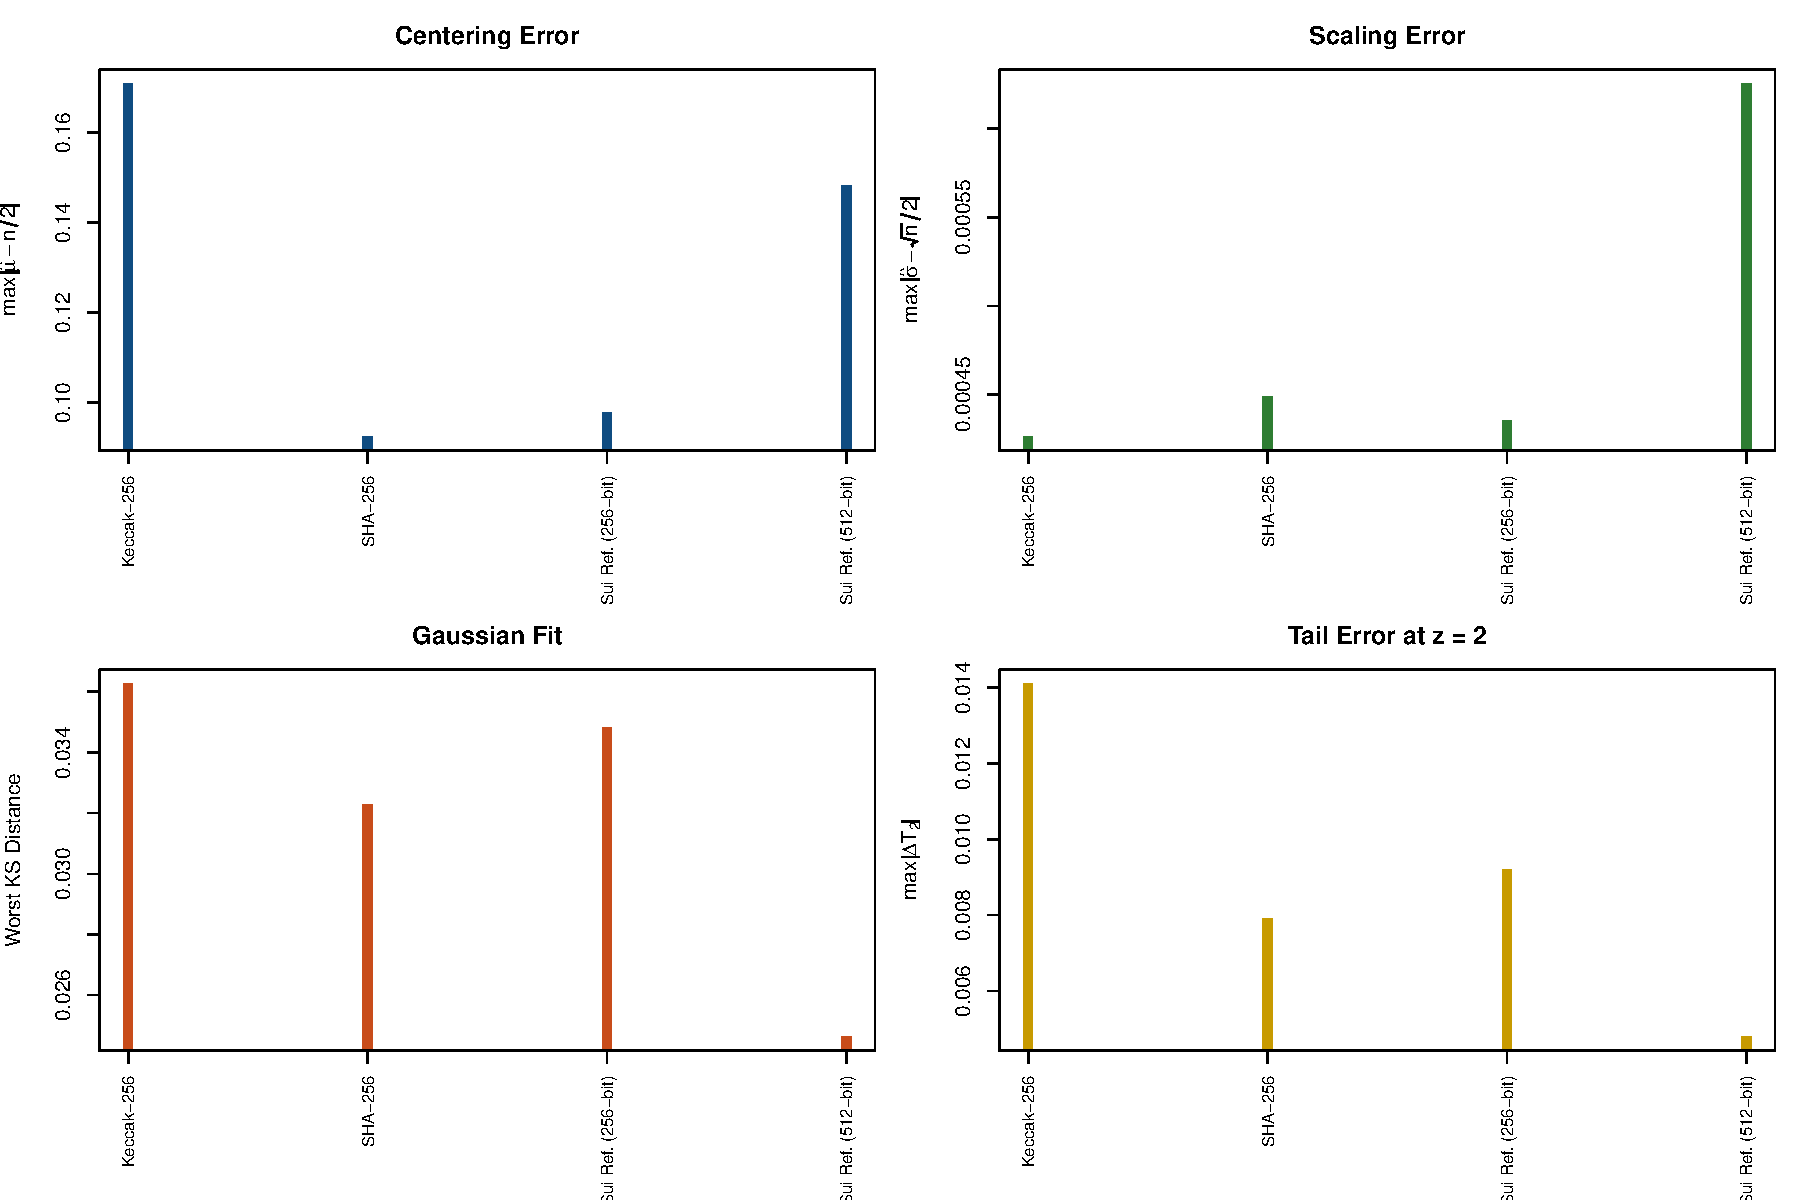
\includegraphics[width=\textwidth]{NumericalStudy/figures/cross_vm_overview.pdf}
\caption{Cross-VM summary of worst normalization and Gaussian-fit diagnostics
across the tested primitives and widths.}
\label{fig:cross-vm-overview}
\end{figure}

\begin{table}[htbp]
\centering
\small
\begin{tabular}{lrrrrrr}
\hline
Primitive & $n$ & $|\Delta\mu|$ & $|\Delta\sigma|$ & KS & $|\Delta T_2|$ & Max $|\rho_h|$ \\
\hline
Keccak-256 & 256 & 0.1708 & 0.0004 & 0.0363 & 0.0141 & 0.0354 \\
SHA-256 & 256 & 0.0924 & 0.0004 & 0.0323 & 0.0079 & 0.0286 \\
Fair-bit control (256-bit) & 256 & 0.0977 & 0.0004 & 0.0348 & 0.0092 & 0.0253 \\
Fair-bit control (512-bit) & 512 & 0.1482 & 0.0006 & 0.0246 & 0.0048 & 0.0218 \\
\hline
\end{tabular}

\caption{Summary diagnostics for the expanded multi-VM study. The sequence
column reports the largest absolute autocorrelation observed in repeated-output
chains up to lag $30$.}
\label{tab:cross-vm-summary}
\end{table}

Figure~\ref{fig:cross-vm-dependence} shows that the corresponding dependence
diagnostics remain small as well. Across the 256-bit hash targets, the worst
sequence lag-1 correlation is about $0.023$ and the worst sequence
autocorrelation up to lag $30$ is about $0.035$. In the 512-bit Sui reference
case, the worst lag-1 correlation is about $0.008$ and the worst sequence
autocorrelation up to lag $30$ is about $0.022$.

\begin{figure}[htbp]
\centering
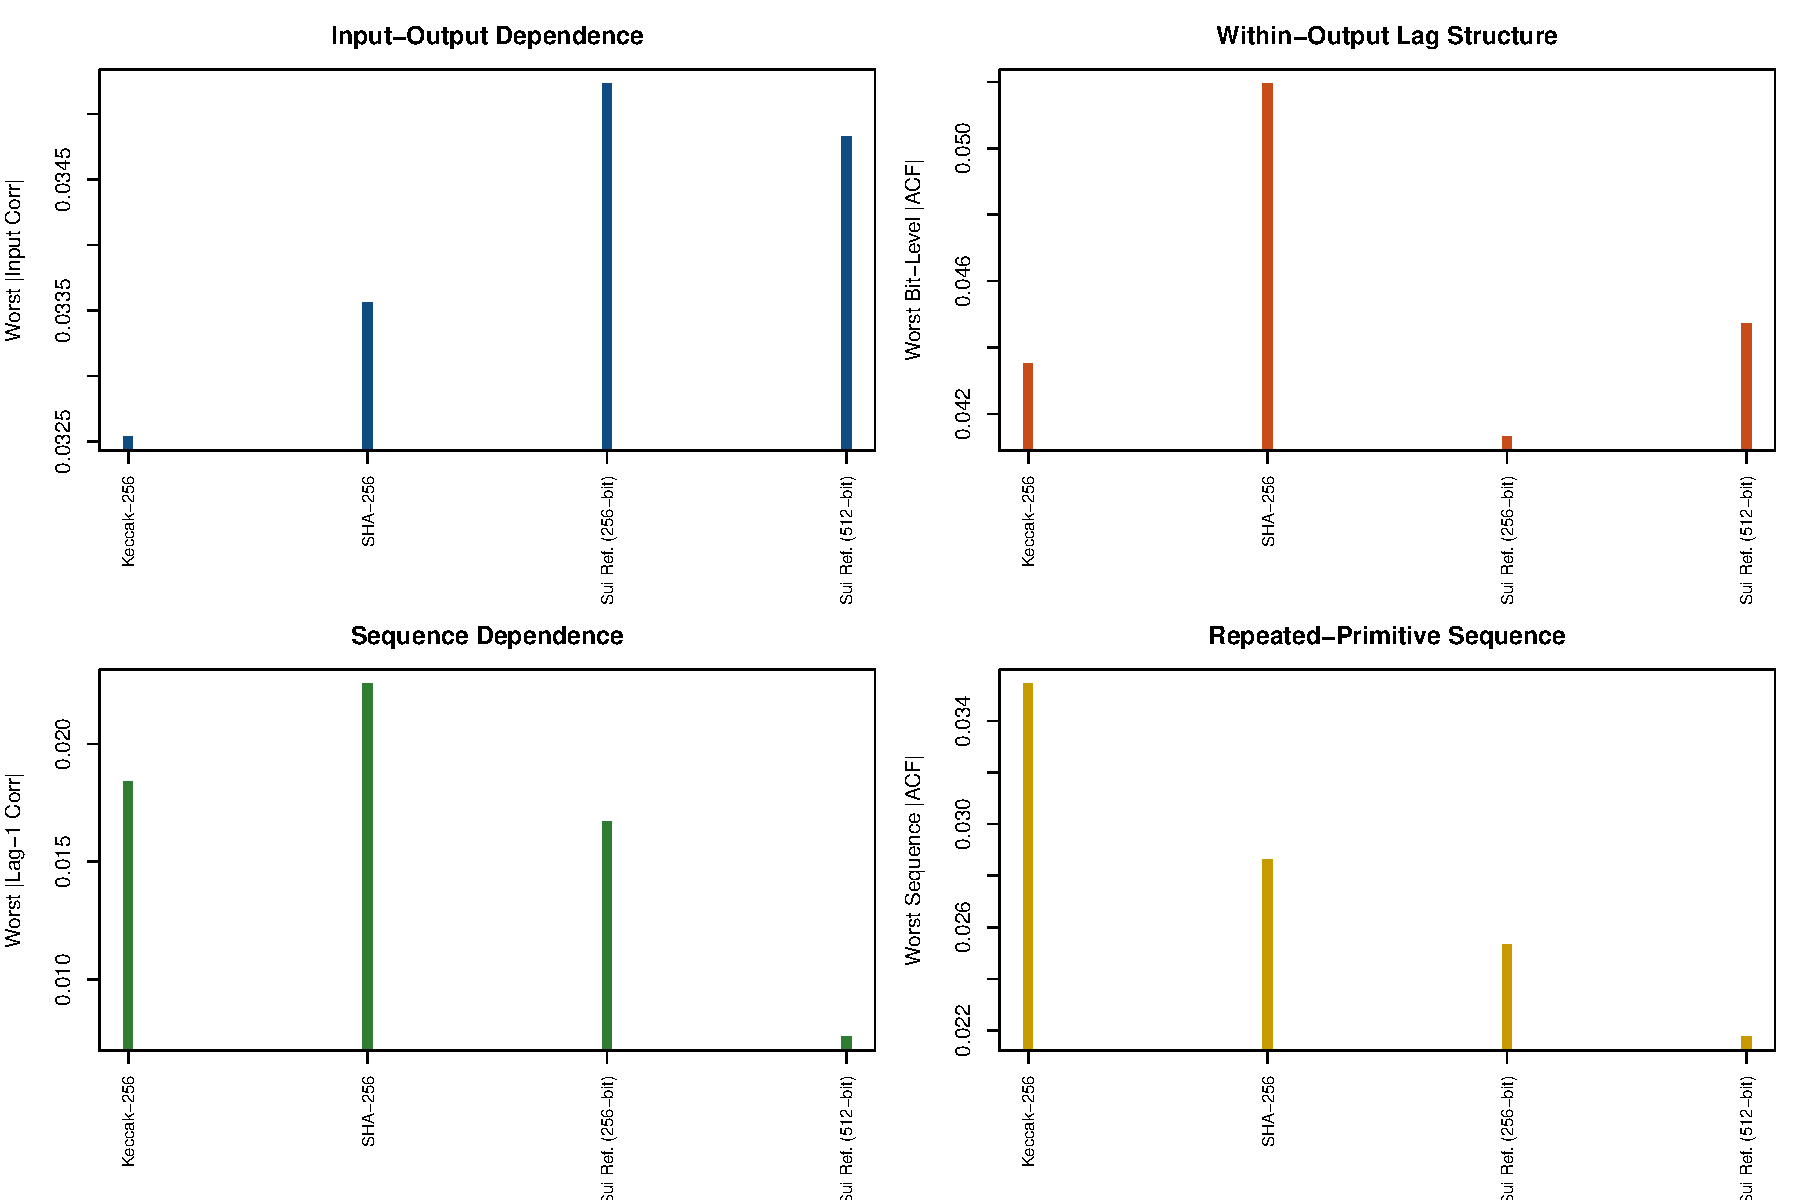
\includegraphics[width=\textwidth]{NumericalStudy/figures/cross_vm_dependence.pdf}
\caption{Cross-VM summary of input-output, within-output, and repeated-sequence
dependence diagnostics.}
\label{fig:cross-vm-dependence}
\end{figure}

The pairwise similarity measures remain highly stable across the tested targets.
Table~\ref{tab:cross-vm-pairwise} shows that the mean Rogers-Tanimoto
similarity stays near $1/3$, the mean Sokal-Michener similarity stays near
$1/2$, and the largest observed absolute phi-correlation remains below about
$0.046$. These values support the claim that the binary-structure diagnostics
do not show a material qualitative change when moving from the original
Keccak-256 study to the broader cross-VM matrix.

\begin{table}[htbp]
\centering
\small
\begin{tabular}{lrrrr}
\hline
Primitive & Mean RT & Mean SM & Mean $|\phi|$ & Max $|\phi|$ \\
\hline
Keccak-256 & 0.3333 & 0.5000 & 0.0080 & 0.0408 \\
SHA-256 & 0.3333 & 0.5000 & 0.0079 & 0.0461 \\
Fair-bit control (256-bit) & 0.3333 & 0.5000 & 0.0079 & 0.0410 \\
Fair-bit control (512-bit) & 0.3333 & 0.5000 & 0.0079 & 0.0441 \\
\hline
\end{tabular}

\caption{Pairwise binary-sequence similarity and correlation diagnostics for the
baseline sequential family in the expanded multi-VM study.}
\label{tab:cross-vm-pairwise}
\end{table}

\section{Uniformity and Dependence Diagnostics}

Figure~\ref{fig:uniformity} shows the empirical mean of each bit with
Bonferroni-adjusted bands. Across all six input families, the bit-wise
probabilities remain close to $0.5$ and do not show an obvious positional
pattern. In the current run, the largest observed absolute deviation
$|\hat p_i - 0.5|$ lies between roughly $0.014$ and $0.019$ across the six
families.

\begin{figure}[htbp]
\centering
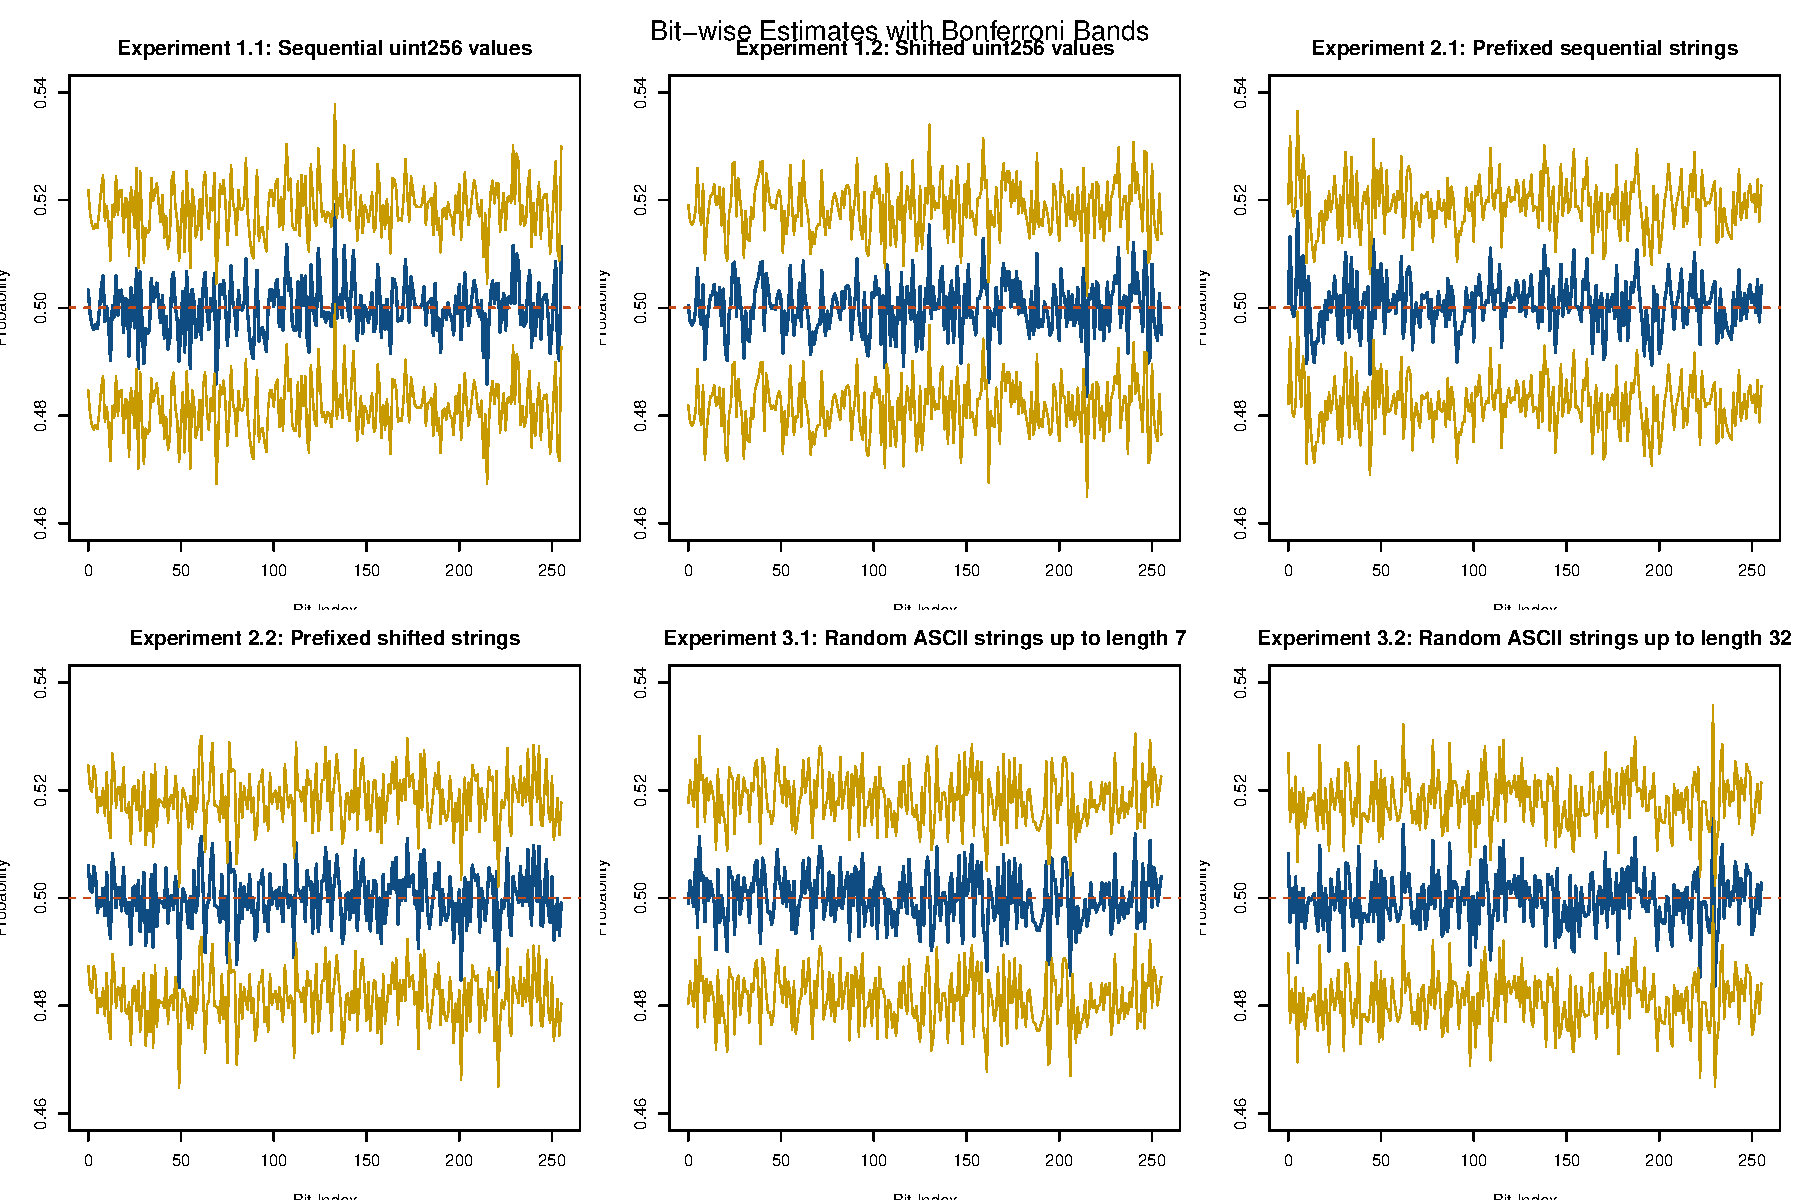
\includegraphics[width=\textwidth]{NumericalStudy/figures/uniformity_panels.pdf}
\caption{Bit-wise empirical means with Bonferroni-adjusted bands for the six
one-shot input families.}
\label{fig:uniformity}
\end{figure}

Figure~\ref{fig:pairwise} shows pairwise similarity and phi-correlation
diagnostics for all $\binom{256}{2}$ bit pairs in the baseline sequential
integer experiment. The phi-correlation distribution is centered near zero, and
the similarity measures stay close to their fair-coin baselines. This is useful
evidence against simple pairwise dependence, though not a proof that higher
order dependence is absent.

\begin{figure}[htbp]
\centering
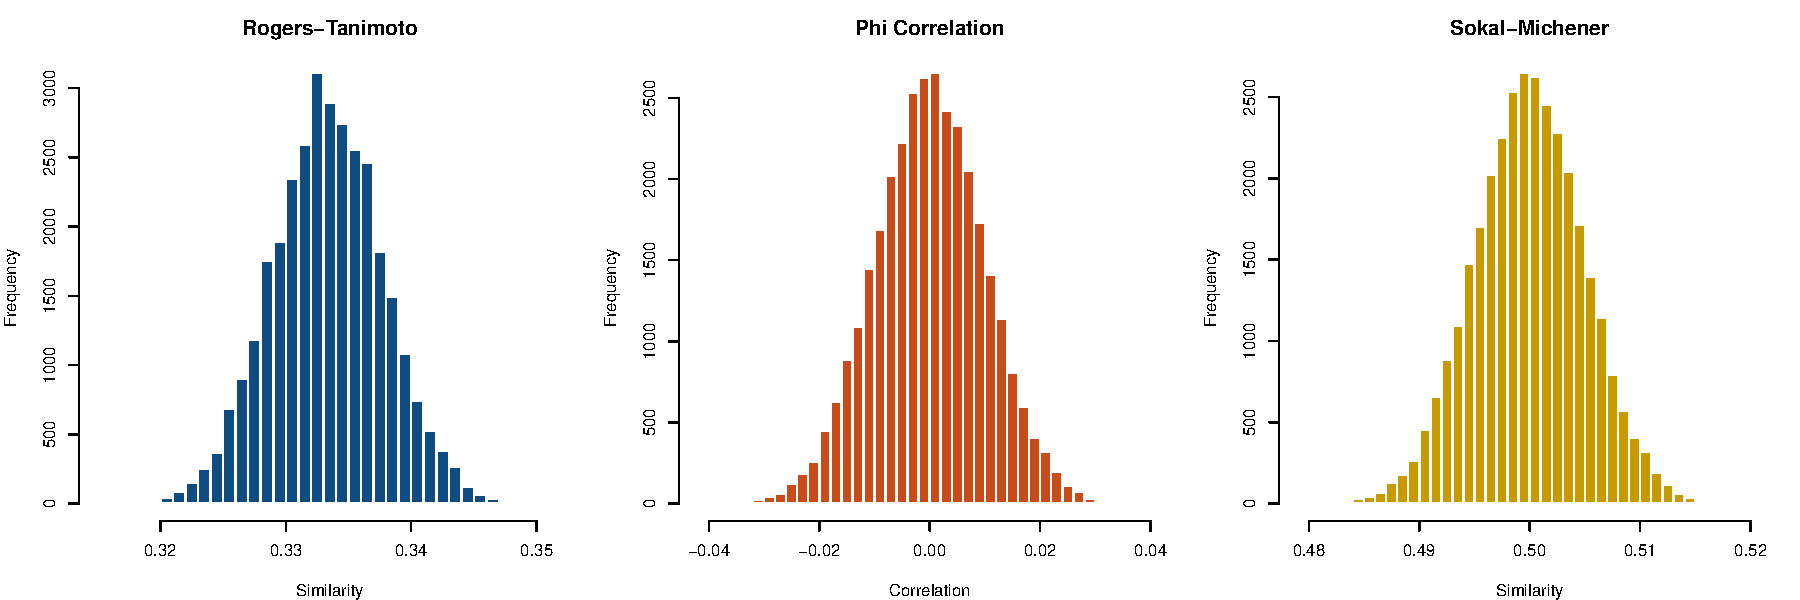
\includegraphics[width=\textwidth]{NumericalStudy/figures/pairwise_metrics.pdf}
\caption{Pairwise similarity and correlation diagnostics for the baseline
sequential integer experiment.}
\label{fig:pairwise}
\end{figure}

Figure~\ref{fig:input-corr} studies whether simple input order survives hashing
in the sequential families. The observed input-bit correlations fluctuate
tightly around zero with no persistent structure by bit position. In this run,
the largest absolute input-bit correlation is about $0.033$.

\begin{figure}[htbp]
\centering
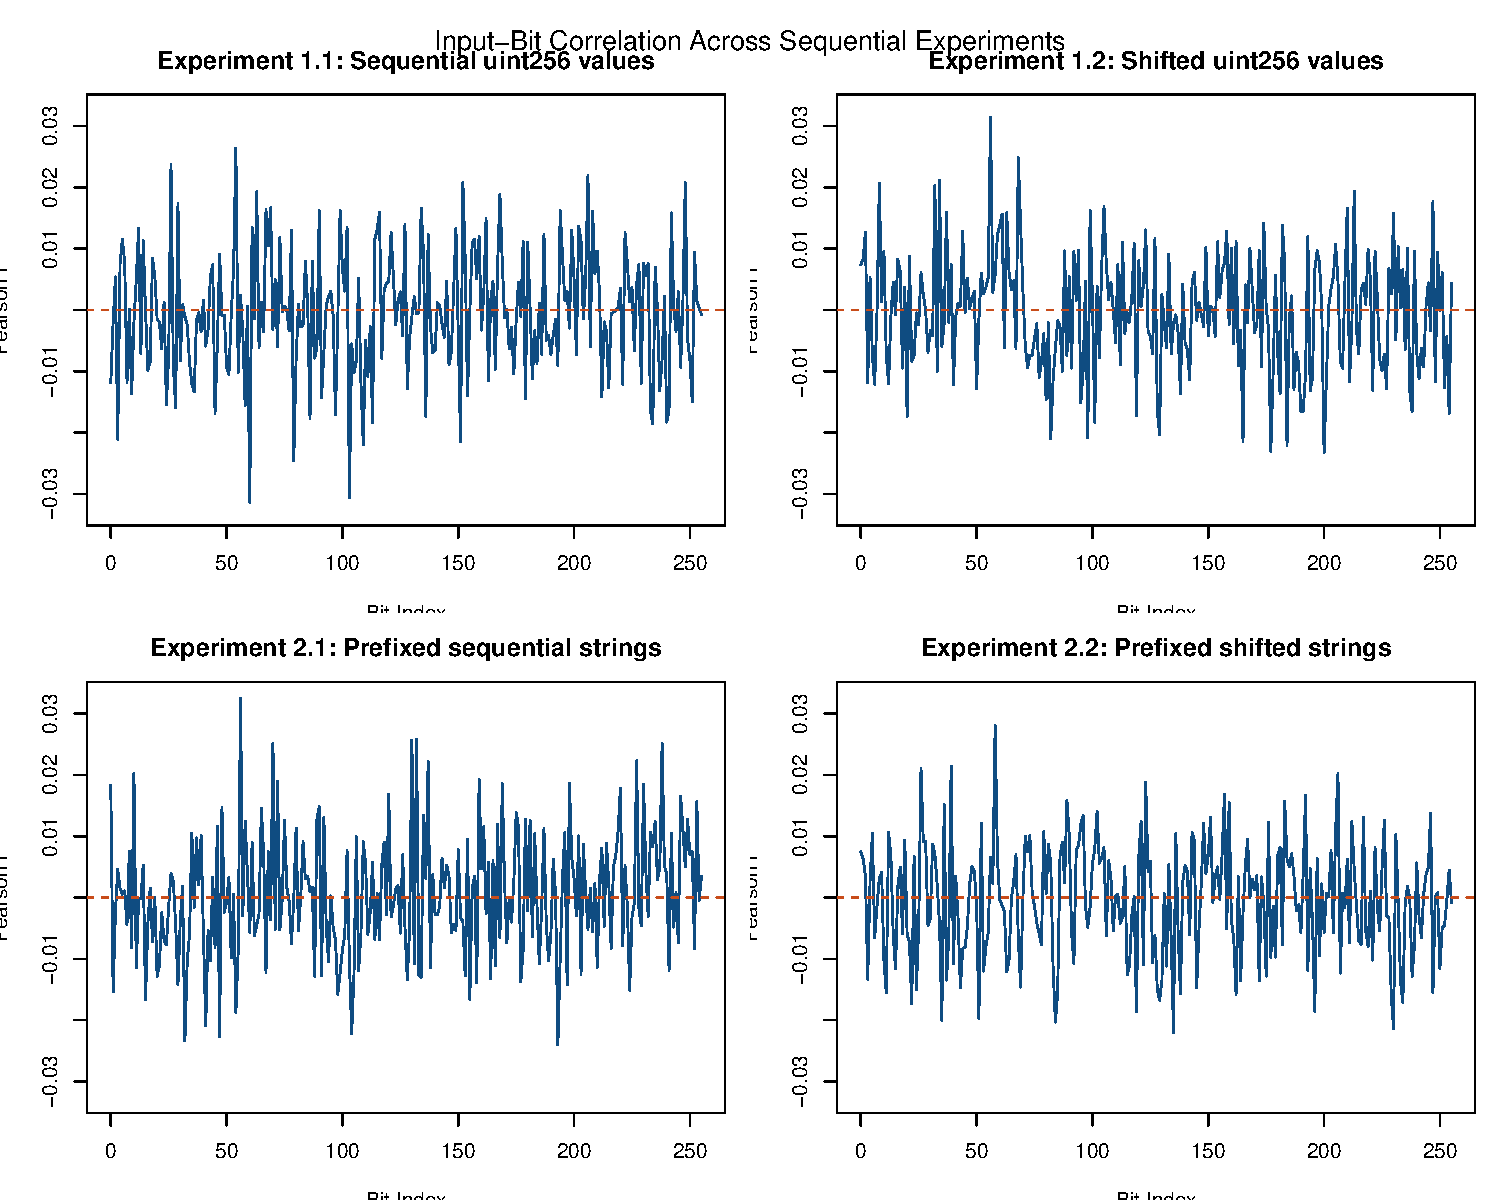
\includegraphics[width=0.92\textwidth]{NumericalStudy/figures/input_correlation_panels.pdf}
\caption{Pearson correlation between input index and each output bit for the
sequential input families.}
\label{fig:input-corr}
\end{figure}

Figure~\ref{fig:bit-acf} summarizes bit-level autocorrelation for lags $1$
through $30$ in the sequential experiments. The largest observed maximum
absolute autocorrelation in the current run is below $0.044$, again suggesting
that simple short-lag structure is weak in the tested regimes.

\begin{figure}[htbp]
\centering
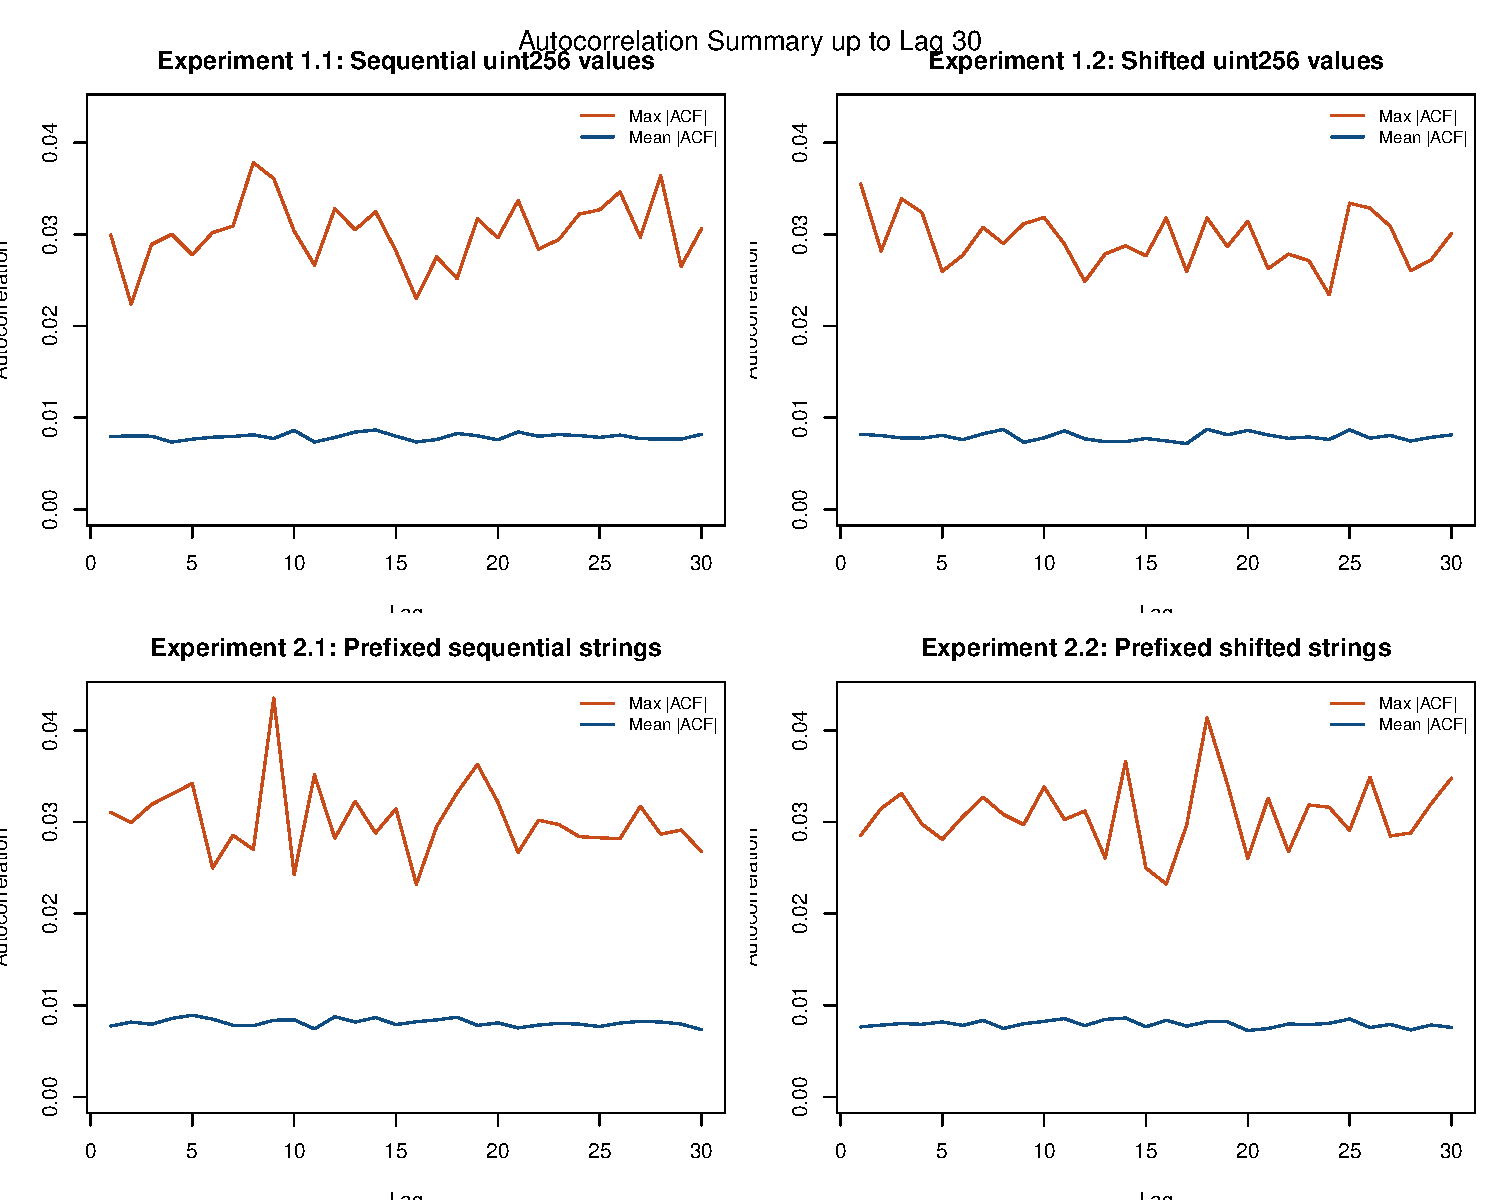
\includegraphics[width=0.92\textwidth]{NumericalStudy/figures/autocorrelation_panels.pdf}
\caption{Mean and maximum absolute bit-level autocorrelation by lag for the
sequential input families.}
\label{fig:bit-acf}
\end{figure}

\section{Normalization and Gaussian-Fit Diagnostics}

The practical Solidity normalization is based on the fixed constants $128$ and
$8$, so the first numerical question is whether the empirical bit model implies
centering and scaling close to
\[
\hat\mu = \sum_{i=1}^{256} \hat p_i \approx 128,
\qquad
\hat\sigma = \sqrt{\sum_{i=1}^{256} \hat p_i(1-\hat p_i)} \approx 8.
\]
Figure~\ref{fig:normalization} and Table~\ref{tab:normalization} show that this
is indeed the case for all six one-shot families. In the present run, the
largest absolute deviation in $\hat\mu$ is about $0.171$, while the largest
absolute deviation in $\hat\sigma$ is below $0.001$.

\begin{figure}[htbp]
\centering
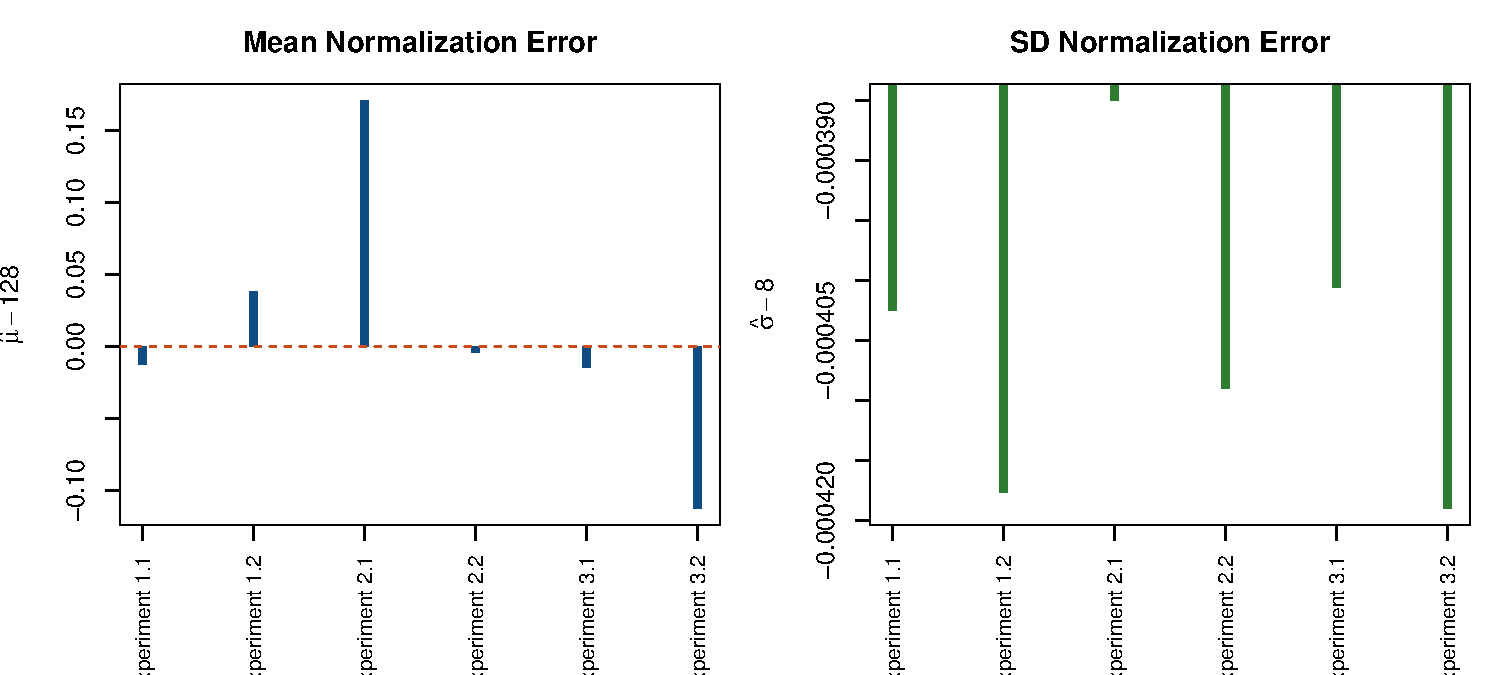
\includegraphics[width=0.92\textwidth]{NumericalStudy/figures/normalization_errors.pdf}
\caption{Empirical deviations of $(\hat\mu, \hat\sigma)$ from the practical
constants $(128, 8)$.}
\label{fig:normalization}
\end{figure}

\begin{table}[htbp]
\centering
\small
\begin{tabular}{lrrrrrr}
\hline
Experiment & $\hat\mu$ & $\hat\mu-128$ & $(\hat\mu-128)/8$ & $\hat\sigma$ & $s_S$ & $s_S^2/\hat\sigma^2$ \\
\hline
Experiment 1.1 & 127.9873 & -0.0127 & -0.0016 & 7.9996 & 7.9854 & 0.9964 \\
Experiment 1.2 & 128.0384 & 0.0384 & 0.0048 & 7.9996 & 7.9520 & 0.9881 \\
Experiment 2.1 & 128.1708 & 0.1708 & 0.0213 & 7.9996 & 8.0663 & 1.0167 \\
Experiment 2.2 & 127.9960 & -0.0040 & -0.0005 & 7.9996 & 8.0182 & 1.0047 \\
Experiment 3.1 & 127.9854 & -0.0146 & -0.0018 & 7.9996 & 7.9888 & 0.9973 \\
Experiment 3.2 & 127.8874 & -0.1126 & -0.0141 & 7.9996 & 7.9731 & 0.9934 \\
\hline
\end{tabular}

\caption{Estimated centering and scaling implied by the empirical bit
probabilities.}
\label{tab:normalization}
\end{table}

Figure~\ref{fig:cdf} compares the empirical popcount CDF to the Gaussian CDF
with mean $128$ and standard deviation $8$. The fit is already visually close.
Figures~\ref{fig:qq} and \ref{fig:tails} extend that comparison with QQ plots
and two-sided tail probabilities for all six one-shot input families.

\begin{figure}[htbp]
\centering
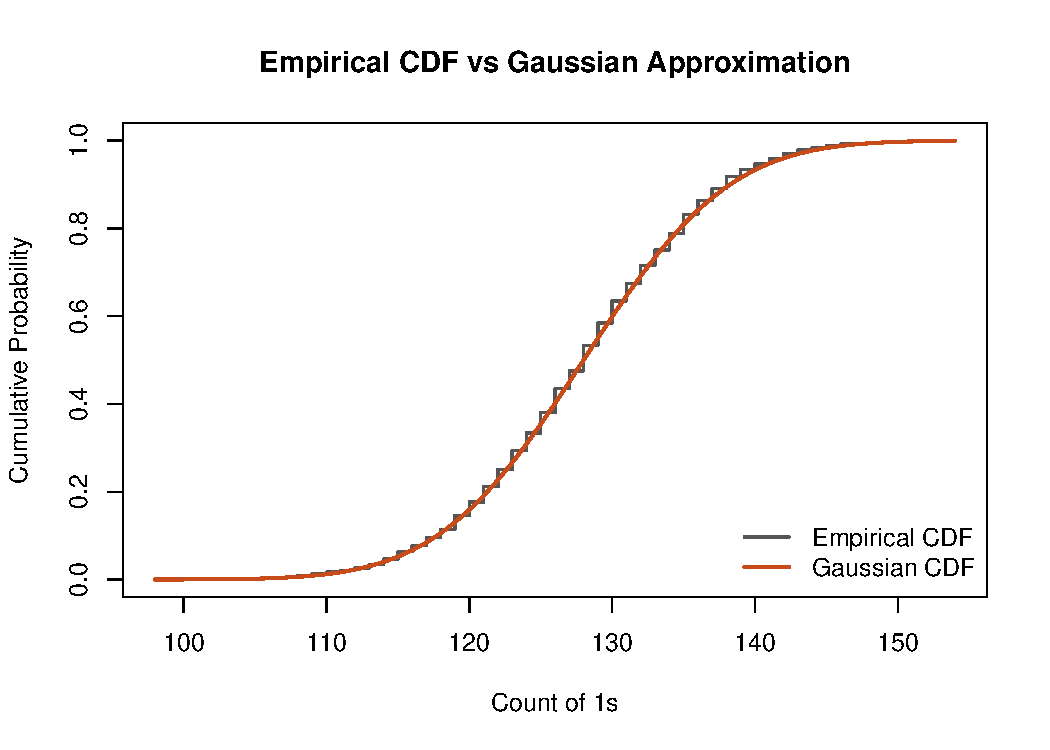
\includegraphics[width=0.78\textwidth]{NumericalStudy/figures/popcount_cdf.pdf}
\caption{Empirical CDF of the popcount against the Gaussian CDF with mean $128$
and standard deviation $8$.}
\label{fig:cdf}
\end{figure}

\begin{figure}[htbp]
\centering
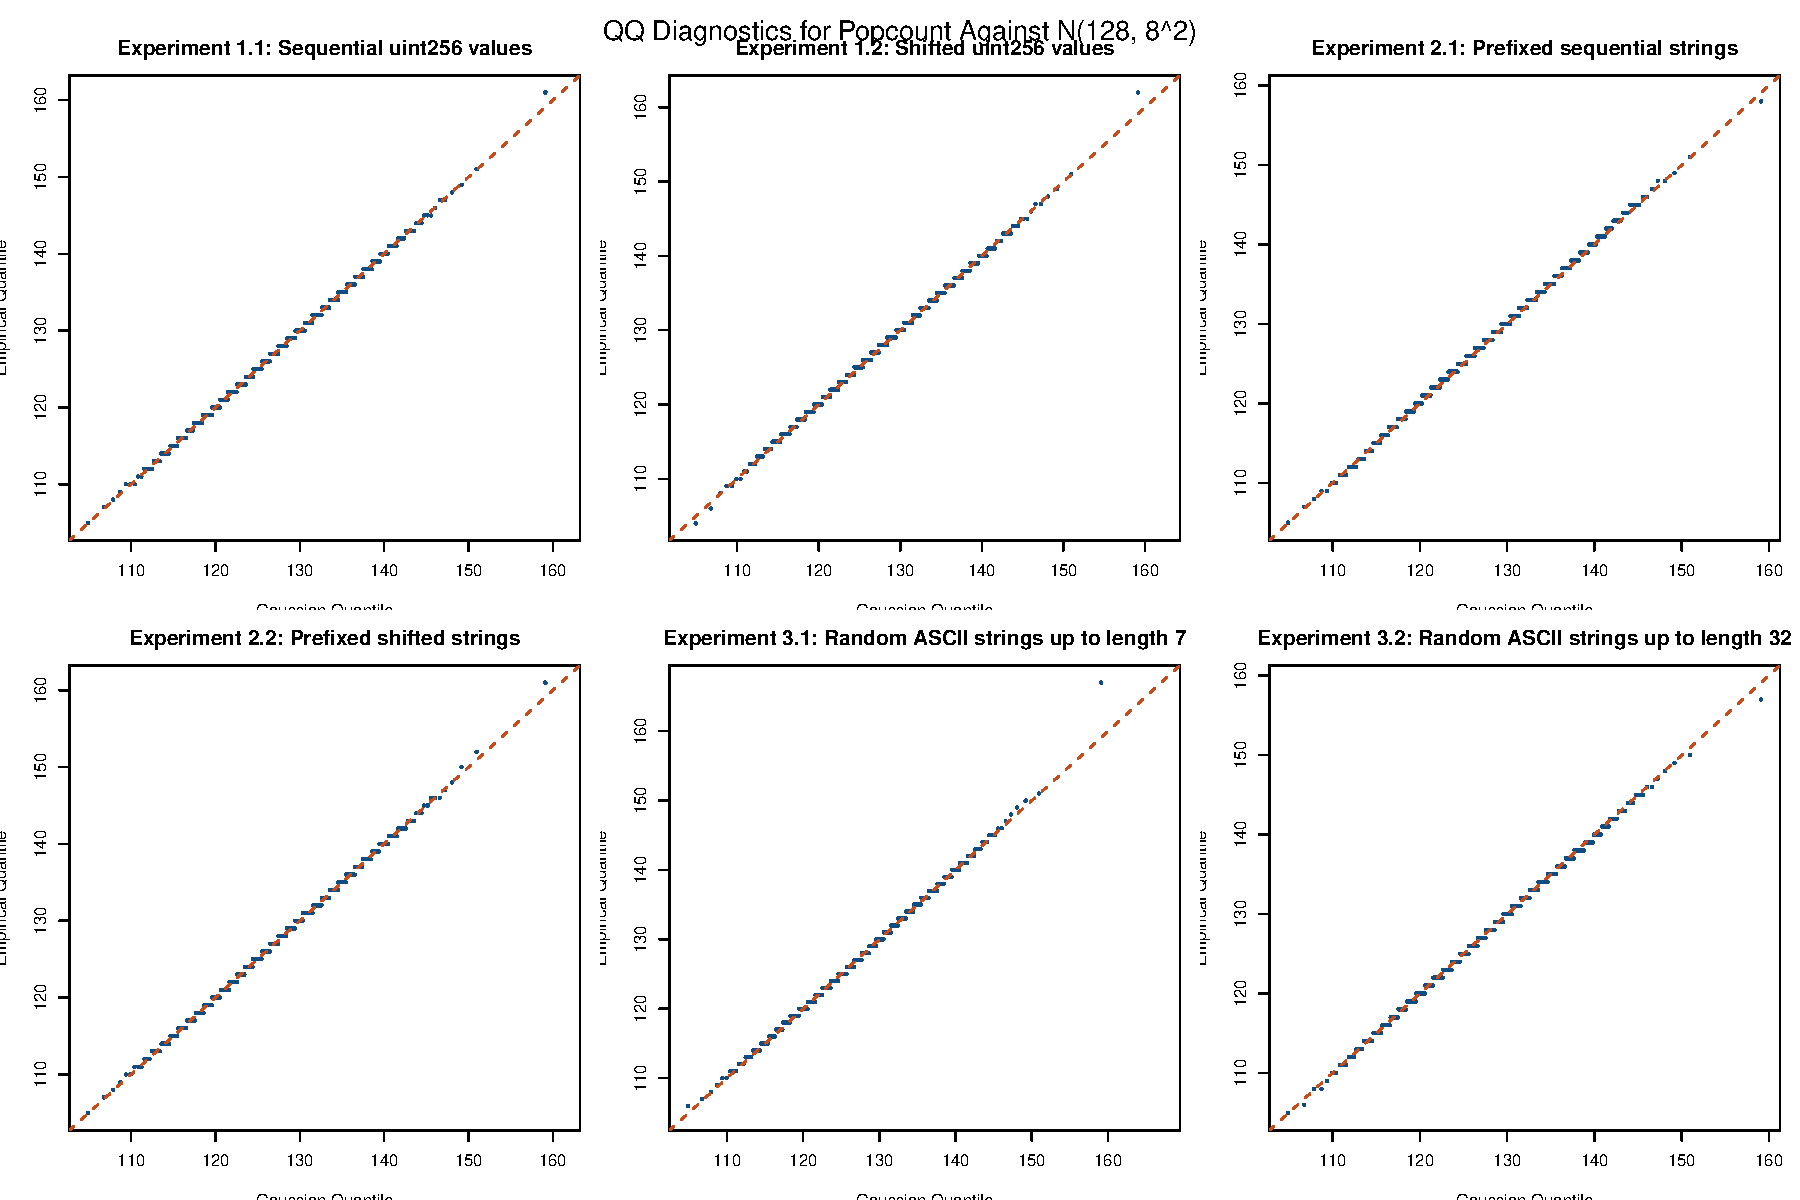
\includegraphics[width=\textwidth]{NumericalStudy/figures/popcount_qq_panels.pdf}
\caption{QQ diagnostics comparing empirical popcount quantiles to the quantiles
of $N(128,8^2)$.}
\label{fig:qq}
\end{figure}

\begin{figure}[htbp]
\centering
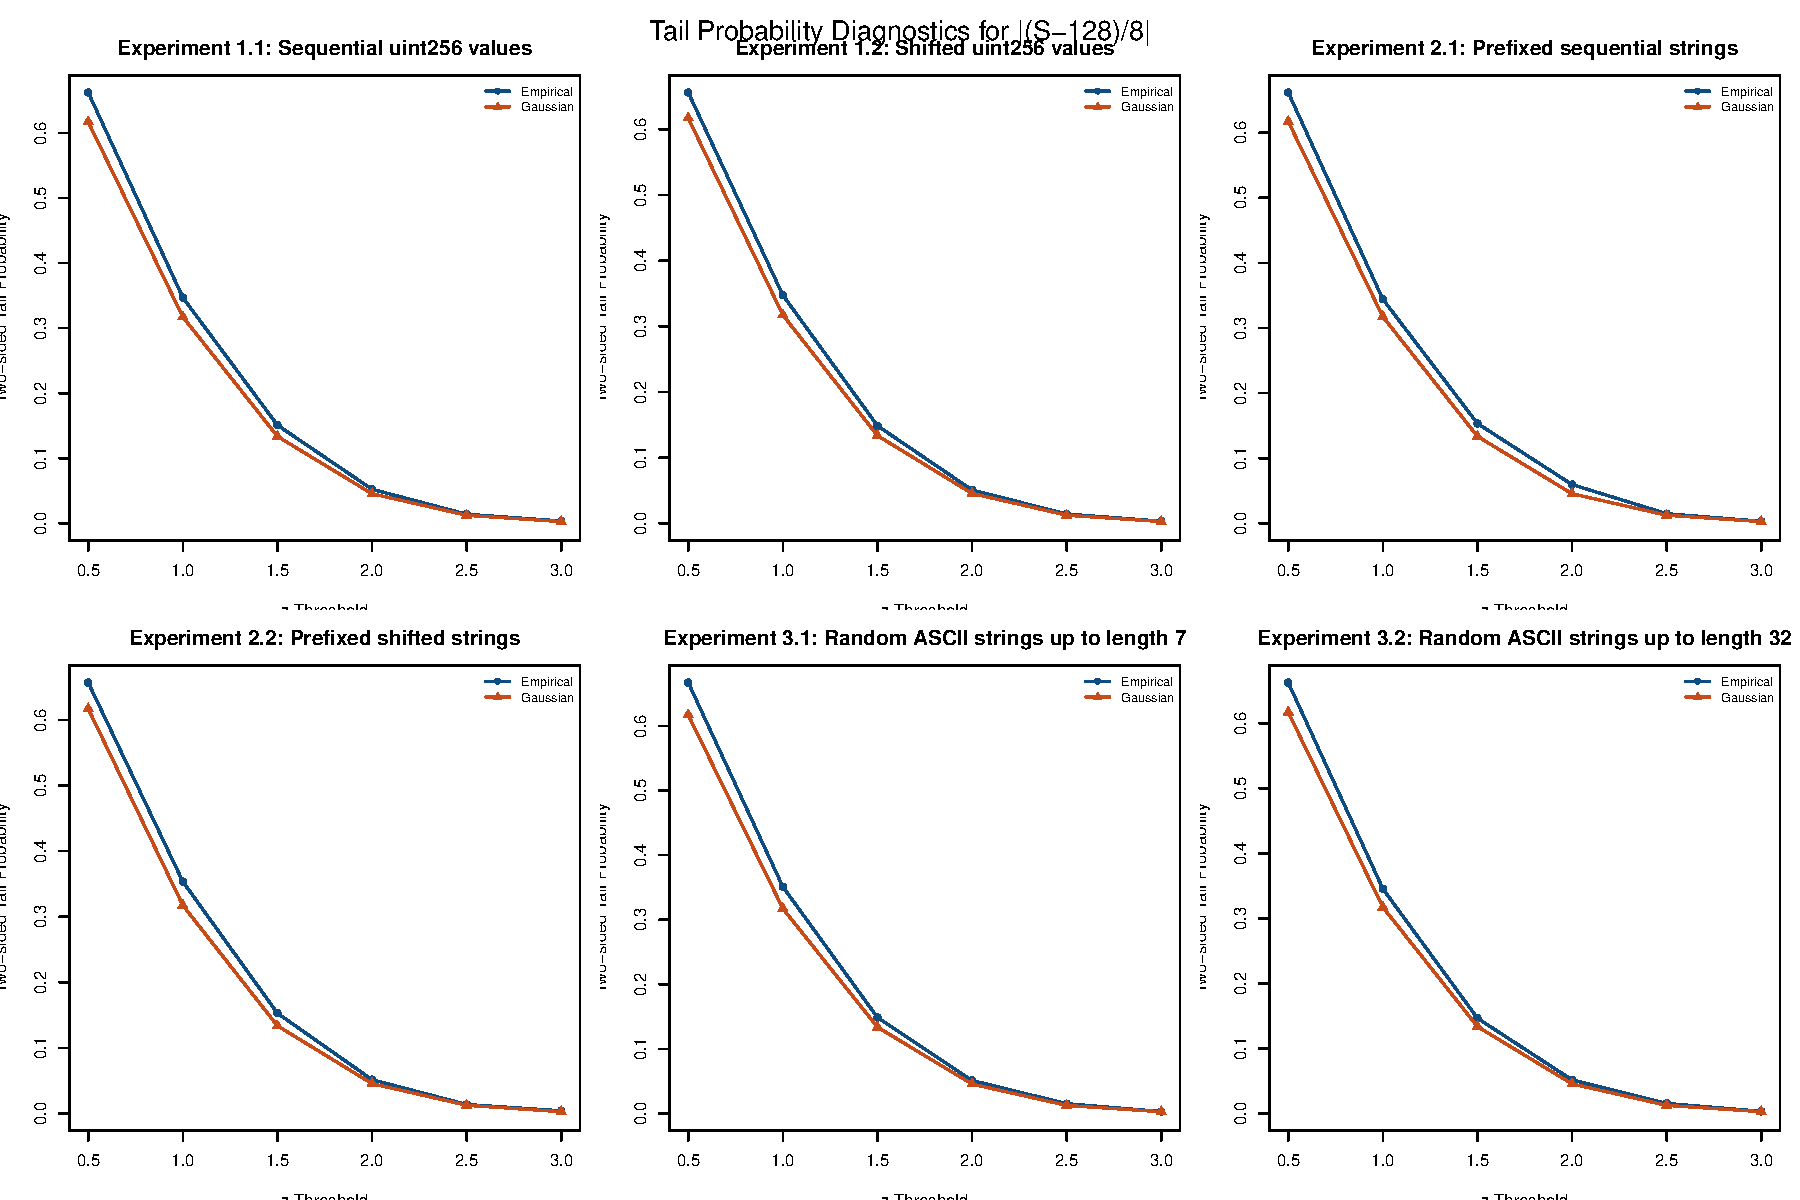
\includegraphics[width=\textwidth]{NumericalStudy/figures/popcount_tail_panels.pdf}
\caption{Empirical and Gaussian two-sided tail probabilities for the
standardized popcount.}
\label{fig:tails}
\end{figure}

Table~\ref{tab:distribution} summarizes the Gaussian fit using the
Kolmogorov-Smirnov distance, a Wasserstein-1 distance, skewness, excess
kurtosis, and the absolute two-sided tail error at $z=2$. In the current run,
the Kolmogorov-Smirnov distance lies between roughly $0.028$ and $0.036$,
while the absolute tail error at $z=2$ lies between roughly $0.005$ and
$0.014$.

\begin{table}[htbp]
\centering
\small
\begin{tabular}{lrrrrrrr}
\hline
Experiment & KS$_{\mathcal N}$ & KS$_{\mathrm{Bin}}$ & $W_1^{\mathcal N}$ & $W_1^{\mathrm{Bin}}$ & Skewness & Excess Kurtosis & $|\Delta T_2|$ \\
\hline
Experiment 1.1 & 0.0282 & 0.0036 & 0.2546 & 0.0490 & 0.0007 & -0.0153 & 0.0069 \\
Experiment 1.2 & 0.0311 & 0.0062 & 0.2624 & 0.0838 & -0.0273 & 0.0419 & 0.0053 \\
Experiment 2.1 & 0.0363 & 0.0117 & 0.2924 & 0.1927 & -0.0137 & 0.0437 & 0.0141 \\
Experiment 2.2 & 0.0288 & 0.0052 & 0.2591 & 0.0669 & 0.0019 & 0.0175 & 0.0060 \\
Experiment 3.1 & 0.0329 & 0.0090 & 0.2684 & 0.0972 & 0.0602 & 0.0009 & 0.0055 \\
Experiment 3.2 & 0.0302 & 0.0067 & 0.2695 & 0.1129 & -0.0235 & 0.0000 & 0.0061 \\
\hline
\end{tabular}

\caption{Finite-sample diagnostics for the Gaussian approximation to the
popcount.}
\label{tab:distribution}
\end{table}

\section{Repeated-Hash Sequence Diagnostics}

The previous sections study isolated hash outputs. The actual generator,
however, is consumed as a sequence. The next question is therefore whether the
recursive map
\[
H_{t+1} = \texttt{keccak256}(H_t)
\]
introduces visible short-lag structure into the popcount sequence
\[
S_t = \text{number of 1's in } H_t.
\]

Figure~\ref{fig:seq-acf} shows the autocorrelation of $S_t$ for four
representative repeated-hash chains and for lags $1$ through $30$.
Figure~\ref{fig:seq-scatter} plots $S_t$ against $S_{t+1}$ for the same chains.
The visual impression is that these chains do not display obvious short-lag
structure. In the current run, the lag-1 correlation lies between roughly
$0.001$ and $0.018$, while the maximum absolute autocorrelation through lag $30$
lies between roughly $0.023$ and $0.035$.

\begin{figure}[htbp]
\centering
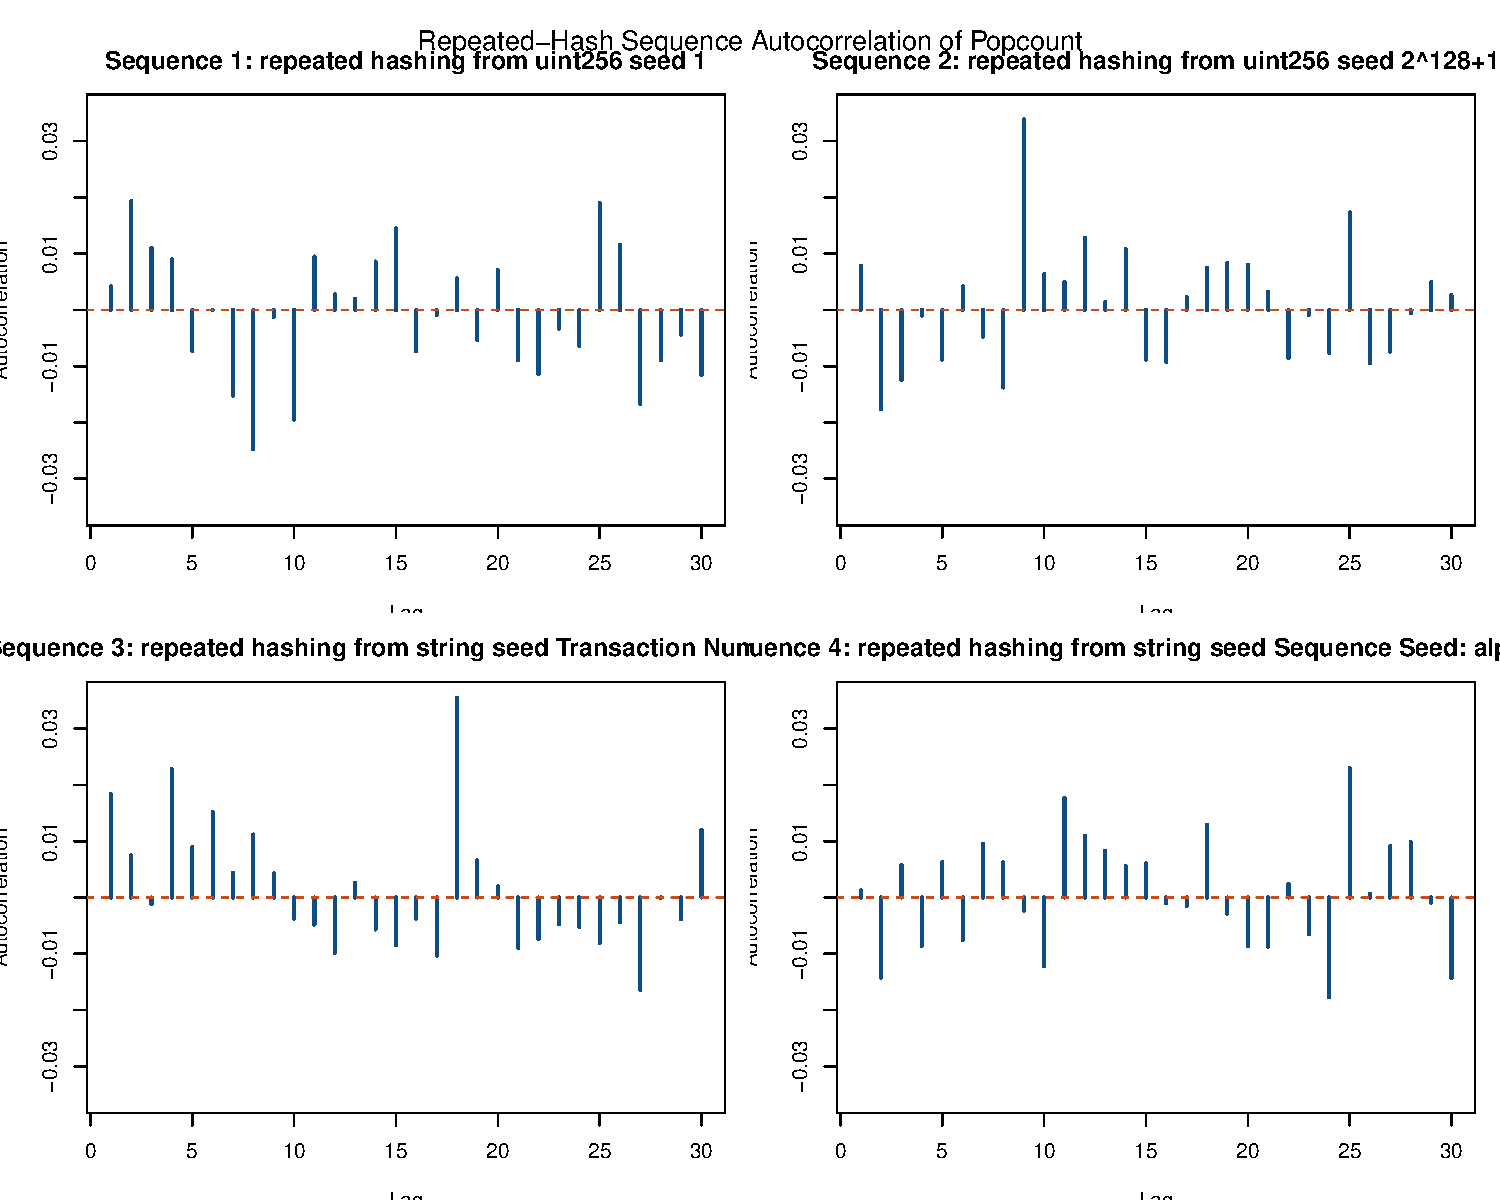
\includegraphics[width=0.92\textwidth]{NumericalStudy/figures/sequence_acf_panels.pdf}
\caption{Autocorrelation of the popcount sequence for four repeated-hash
chains.}
\label{fig:seq-acf}
\end{figure}

\begin{figure}[htbp]
\centering
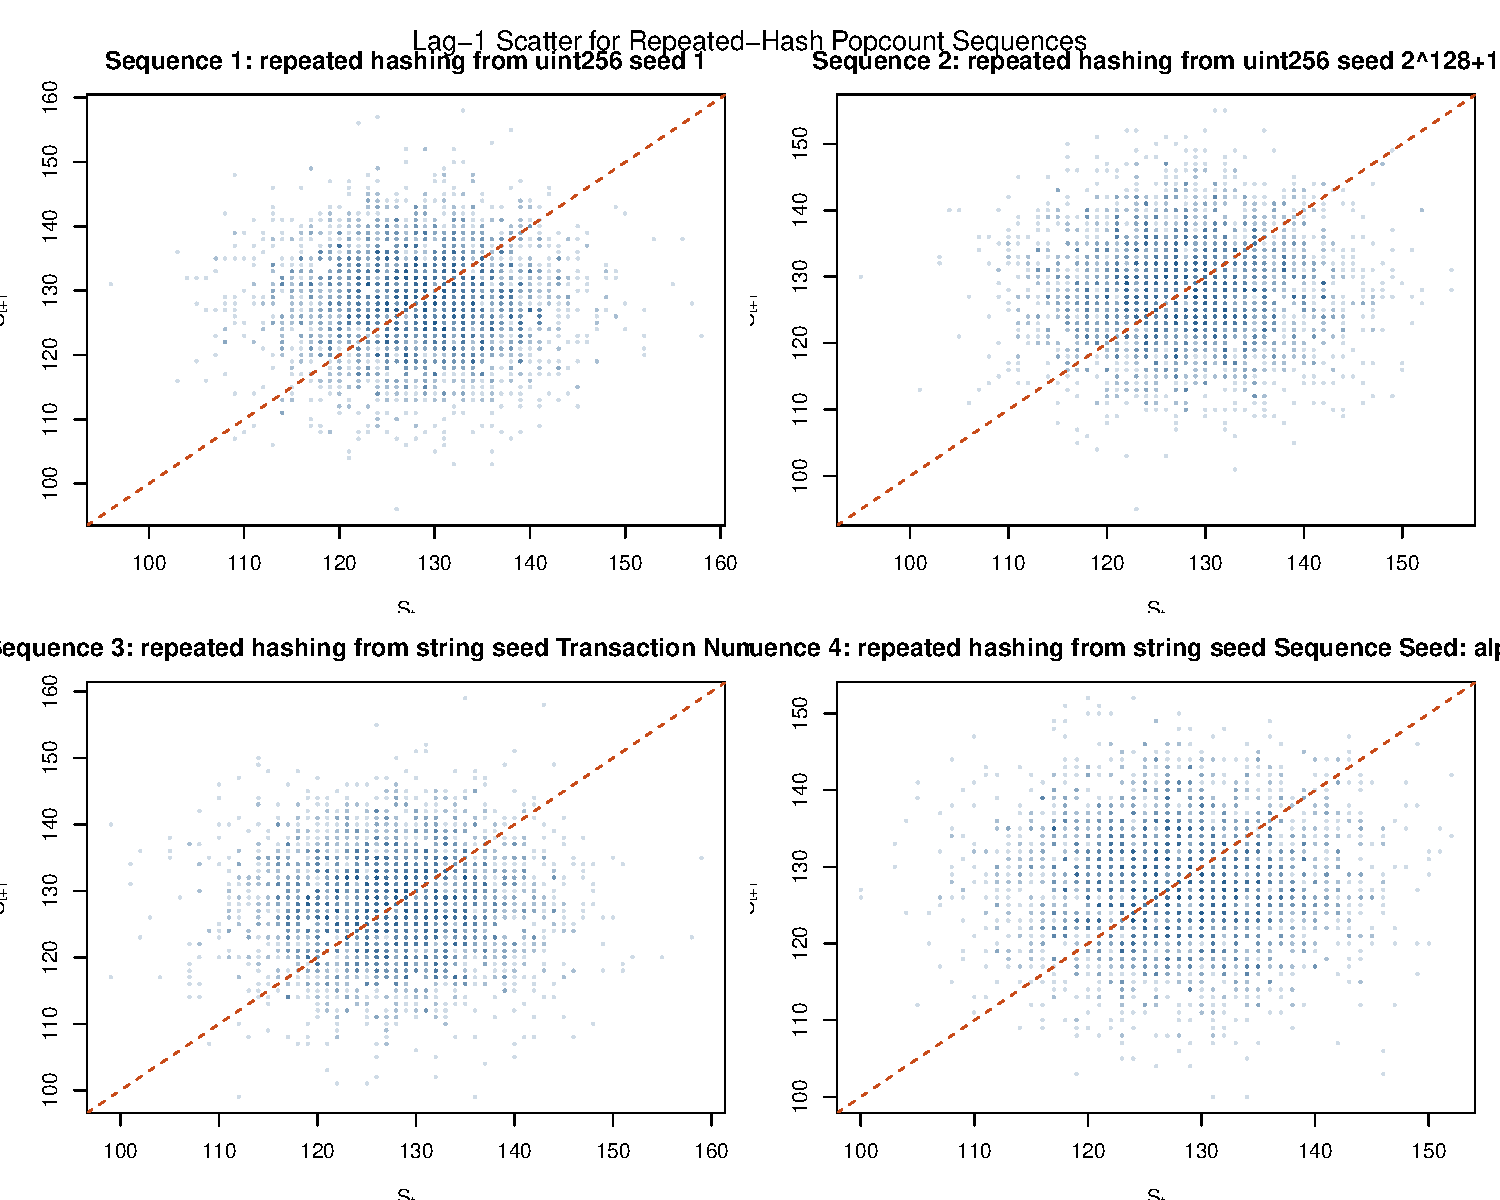
\includegraphics[width=0.92\textwidth]{NumericalStudy/figures/sequence_scatter_panels.pdf}
\caption{Lag-1 scatter plots for repeated-hash popcount sequences.}
\label{fig:seq-scatter}
\end{figure}

Table~\ref{tab:sequence} summarizes the same study by reporting the mean and
standard deviation of the popcount sequence, the lag-1 correlation, and the
largest absolute autocorrelation up to lag $30$. The associated runs-test
$z$-scores are also modest in the current run, which is again compatible with
the absence of obvious short-lag dependence for the tested seeds.

\begin{table}[htbp]
\centering
\small
\begin{tabular}{lrrrrrr}
\hline
Sequence & Mean Count & SD Count & Lag-1 Corr & Max $|\rho_h|$ & Runs $z$ & $|\Delta T_2|$ \\
\hline
Sequence 1 & 127.9579 & 7.9600 & 0.0042 & 0.0248 & 0.1287 & 0.0027 \\
Sequence 2 & 128.0153 & 7.9580 & 0.0079 & 0.0339 & -0.1537 & 0.0083 \\
Sequence 3 & 128.0109 & 7.9452 & 0.0184 & 0.0354 & -1.4950 & 0.0047 \\
Sequence 4 & 127.8900 & 7.9386 & 0.0013 & 0.0230 & 0.7849 & 0.0068 \\
\hline
\end{tabular}

\caption{Summary diagnostics for repeated-hash popcount sequences.}
\label{tab:sequence}
\end{table}

\section{On-Chain Implications}

The practical interpretation of the numerical study is straightforward. If the
bit probabilities remain close to $0.5$, then the natural centering and scaling
are already close to $(128,8)$. If the popcount distribution is close to a
Gaussian benchmark at $n=256$, then the integer-scaled Solidity output
\[
125S - 16000
\]
is a plausible discrete approximation to a standard normal draw with three
decimal digits of precision.

This approach is attractive on-chain because it avoids floating-point
operations, trigonometric transforms, and expensive rejection samplers. The
computation reduces to hashing and bit counting. The price of this simplicity is
that the distributional claim is only as strong as the probabilistic model and
the empirical evidence supporting it.

\begin{table}[htbp]
\centering
\small
\begin{tabular}{lrrrrr}
\hline
Experiment & Max $|\hat p_i-0.5|$ & Mean Count & SD Count & Max $|r|$ & Max $|\rho_h|$ \\
\hline
Experiment 1.1 & 0.0192 & 127.9873 & 7.9854 & 0.0314 & 0.0378 \\
Experiment 1.2 & 0.0164 & 128.0384 & 7.9520 & 0.0314 & 0.0355 \\
Experiment 2.1 & 0.0179 & 128.1708 & 8.0663 & 0.0325 & 0.0435 \\
Experiment 2.2 & 0.0166 & 127.9960 & 8.0182 & 0.0281 & 0.0414 \\
Experiment 3.1 & 0.0144 & 127.9854 & 7.9888 & -- & -- \\
Experiment 3.2 & 0.0171 & 127.8874 & 7.9731 & -- & -- \\
\hline
\end{tabular}

\caption{Summary diagnostics across the six one-shot experiments.}
\label{tab:summary}
\end{table}

\section{Scope and Limitations}

\begin{remark}
The numerical study provides empirical support for the modeling assumptions, but
it does not prove full joint independence of the 256 output bits of
\texttt{keccak256}.
\end{remark}

\begin{remark}
Lyapunov's theorem addresses non-identical Bernoulli marginals under
independence. It does not justify the Gaussian approximation if genuine
dependence among the bits is materially present.
\end{remark}

\begin{remark}
The theorem is asymptotic, whereas the intended implementation uses the fixed
value $n=256$. The practical argument therefore depends on both the CLT
heuristic and the finite-sample numerical diagnostics.
\end{remark}

\begin{remark}
The repeated-hash study addresses obvious short-lag structure for a small set of
representative seeds. It should not be read as a proof against all forms of
long-range or adversarially chosen dependence.
\end{remark}

\begin{remark}
This paper is best read as an applied probabilistic construction with empirical
validation. It is not a cryptographic security proof and it does not claim that
the resulting generator is appropriate for every randomness-sensitive use case.
\end{remark}

\section{Conclusion}

The clean statement supported by this paper is the following. Model the
\texttt{keccak256} output bits as independent Bernoulli random variables with
possibly different success probabilities $p_i$. Under that model, the popcount
has a Poisson-binomial distribution, and Lyapunov's central limit theorem
implies that the standardized count is asymptotically Gaussian. The numerical
study then provides empirical support for the practical finite-sample
approximation
\[
\frac{S-128}{8} \approx \mathcal{N}(0,1),
\]
which leads directly to the integer-scaled on-chain representation
\[
125S - 16000.
\]

The empirical evidence remains intentionally modest. It does not prove
independence or certify the generator cryptographically. It does, however, make
the working model substantially harder to dismiss. For the quantities the
generator actually uses, namely the centering, the scaling, the popcount
distribution, and the repeated-hash output sequence, the observed behavior is
close to what the practical Gaussian RNG construction requires. The same method
also has a clear path beyond \texttt{keccak256}: it can be applied to other
VM-exposed primitives, with EVM and Solana as the clearest missing-Gaussian
targets and Sui as a natural native-randomness comparison case.

\end{document}
